\documentclass[ucs,10pt]{beamer}
\mode<presentation>
\hypersetup{pdfpagemode=FullScreen}
\usepackage{subfig}
\usepackage{beamerthemesplit}
\usepackage{beamer_visser_um}
\usepackage{graphicx}

\setlength{\unitlength}{\textwidth}  % measure in textwidths 


\title{Activity Monitoring and Prediction for Humans and NAO Humanoid Robots using 
	Wearable Sensors}
\author{\textbf{Saminda Abeyruwan} and  \textbf{Faisal Sikder} and \textbf{Ubbo Visser} and \textbf{Dilip Sarkar}}
\institute{Department of Computer Science\\ University of Miami \\ \vspace{.25cm}}
\date{May 19, 2015}
\titlegraphic{\putat{-0.52}{-0.15}{\includegraphics[height=1.5cm]{logos/theUlogo}}}


\begin{document}

%%%%%%%%%%%%%%%%%%%%%%%%%%%%%%%%%%%%%%%%%%%%%%%%%%%%%%%%%%%%%


\frame{\titlepage}

\section*{Outline}
\frame{
  \frametitle{Outline}    
  \tableofcontents
}

%%%%%%%%%%%%%%%%%%%%%%%%%%%%%%%%%%%%%%%%%%%%%%%%%%%%%%%%%%%%%

\section{Introduction}
\subsection{Introduction}
\subsection{Motivation}

\subsubsection*{Challenges in activities in human and biped humanoid robots}
\frame{
  \frametitle{Introduction}
  \setbeamercovered{transparent} 
  \begin{block}{Challenges in activities in human and biped humanoid robots}
  	\begin{itemize}
  		\item Activity like jogging, running might cause an accident event such as fall. This might cause damage to the human body or to the structural components of the robot.
  		
  		\item Immediate identification of a fall will allow fast responses, and in case of robots it might be able to corrects its motion to prevent accident.
  		
  		\item Though both human and biped humanoid robots share lots of similar  features, using same framework it never has been tested to use external embedded devices to identify activities on both.
  		
  	\end{itemize}
 
  \end{block}
}

%%%%%%%%%%%%%%%%%%%%%%%%%%%%%%%%%%%%%%%%%%%%%%%%%%%%%%%%%%%%%

\subsubsection*{Motivation}
\frame{
	\frametitle{Motivation}
	\setbeamercovered{transparent} 
	\begin{block}{Motivation}
		 \begin{itemize}
		 	\item Humans and biped humanoid robots have almost identical movements and are  susceptible to similar accidents, we believe that the same set of learning algorithms
		 	are suitable for both groups.
		 	\item We want to use off-the-shelf hardware components to develop our sensing tools.
		 	\item We want to develop a generalized approach for learning and predicting
		 	activities of both groups.
		 	
		 	\item  Detection of falls for both humans and robots within a unified framework;
		 	
		 \end{itemize}
	\end{block}
}

%%%%%%%%%%%%%%%%%%%%%%%%%%%%%%%%%%%%%%%%%%%%%%%%%%%%%%%%%%%%%

\section{Our Approach and Contributions}
\subsection{Devices}
\subsection{Frameworks}

\subsubsection*{Devices}
\frame{
	\frametitle{Our Approach and Contributions}
	\setbeamercovered{transparent} 
	\begin{block}{Devices}
		\begin{itemize}
			\item We have put 
			\begin{enumerate}
			\item Tiva C Series TM4C123G microcontroller board
			\item  A Sensor Hub BoosterPack for sensing 9-axis motion
			\item A CC2533 BoosterPack for wireless networking.
			\end{enumerate}
			\item 
			We have developed a set of software tools to create a framework that allow us
			\begin{enumerate}
				 \item  To setup the WSN, 
				 \item collect data using WSN network, 
				 \item to learn from sample examples, and 
				 \item to monitor and predict events. 
			\end{enumerate} 
		\end{itemize}
		
	\end{block}
}


%%%%%%%%%%%%%%%%%%%%%%%%%%%%%%%%%%%%%%%%%%%%%%%%%%%%%%%%%%%%%

\subsubsection*{Frameworks}
\frame{
	\frametitle{Our Approach and Contributions}
	\setbeamercovered{transparent} 
	\begin{block}{Frameworks}
		\begin{itemize}
			\item Our framework provides generic functionalities to develop applications or rational agents on embedded devices.
			\item The execution paths is ensured using a topologically sorted graph, based on the decision points provided by practitioners.
			\item The framework includes: 
			\begin{enumerate}
			 \item tools to develop modules and representations that execute on the microcontrollers or off-line, 
			\item the methods to access functionalities for physical robots, and 
			\item a real-time visualization system
			\end{enumerate}.
			\item Our development framework, $\mu$Energia (\textit{pronounced as}: ``micro--Energia'' and 
			\textit{site}:
			{http://muenergia.saminda.org}), uses a notion of  {\em modules} and {\em representations} to 
			perform computations.
		\end{itemize}
		
	\end{block}
}



%%%%%%%%%%%%%%%%%%%%%%%%%%%%%%%%%%%%%%%%%%%%%%%%%%%%%%%%%%%%%

\subsubsection*{Frameworks}
\frame{
	\frametitle{Our Approach and Contributions}
	\setbeamercovered{transparent} 
	\begin{block}{Frameworks}
		\begin{figure*}
			\centering
			\includegraphics[width=0.6\textwidth]{figures/graph_structure_def-crop3}
			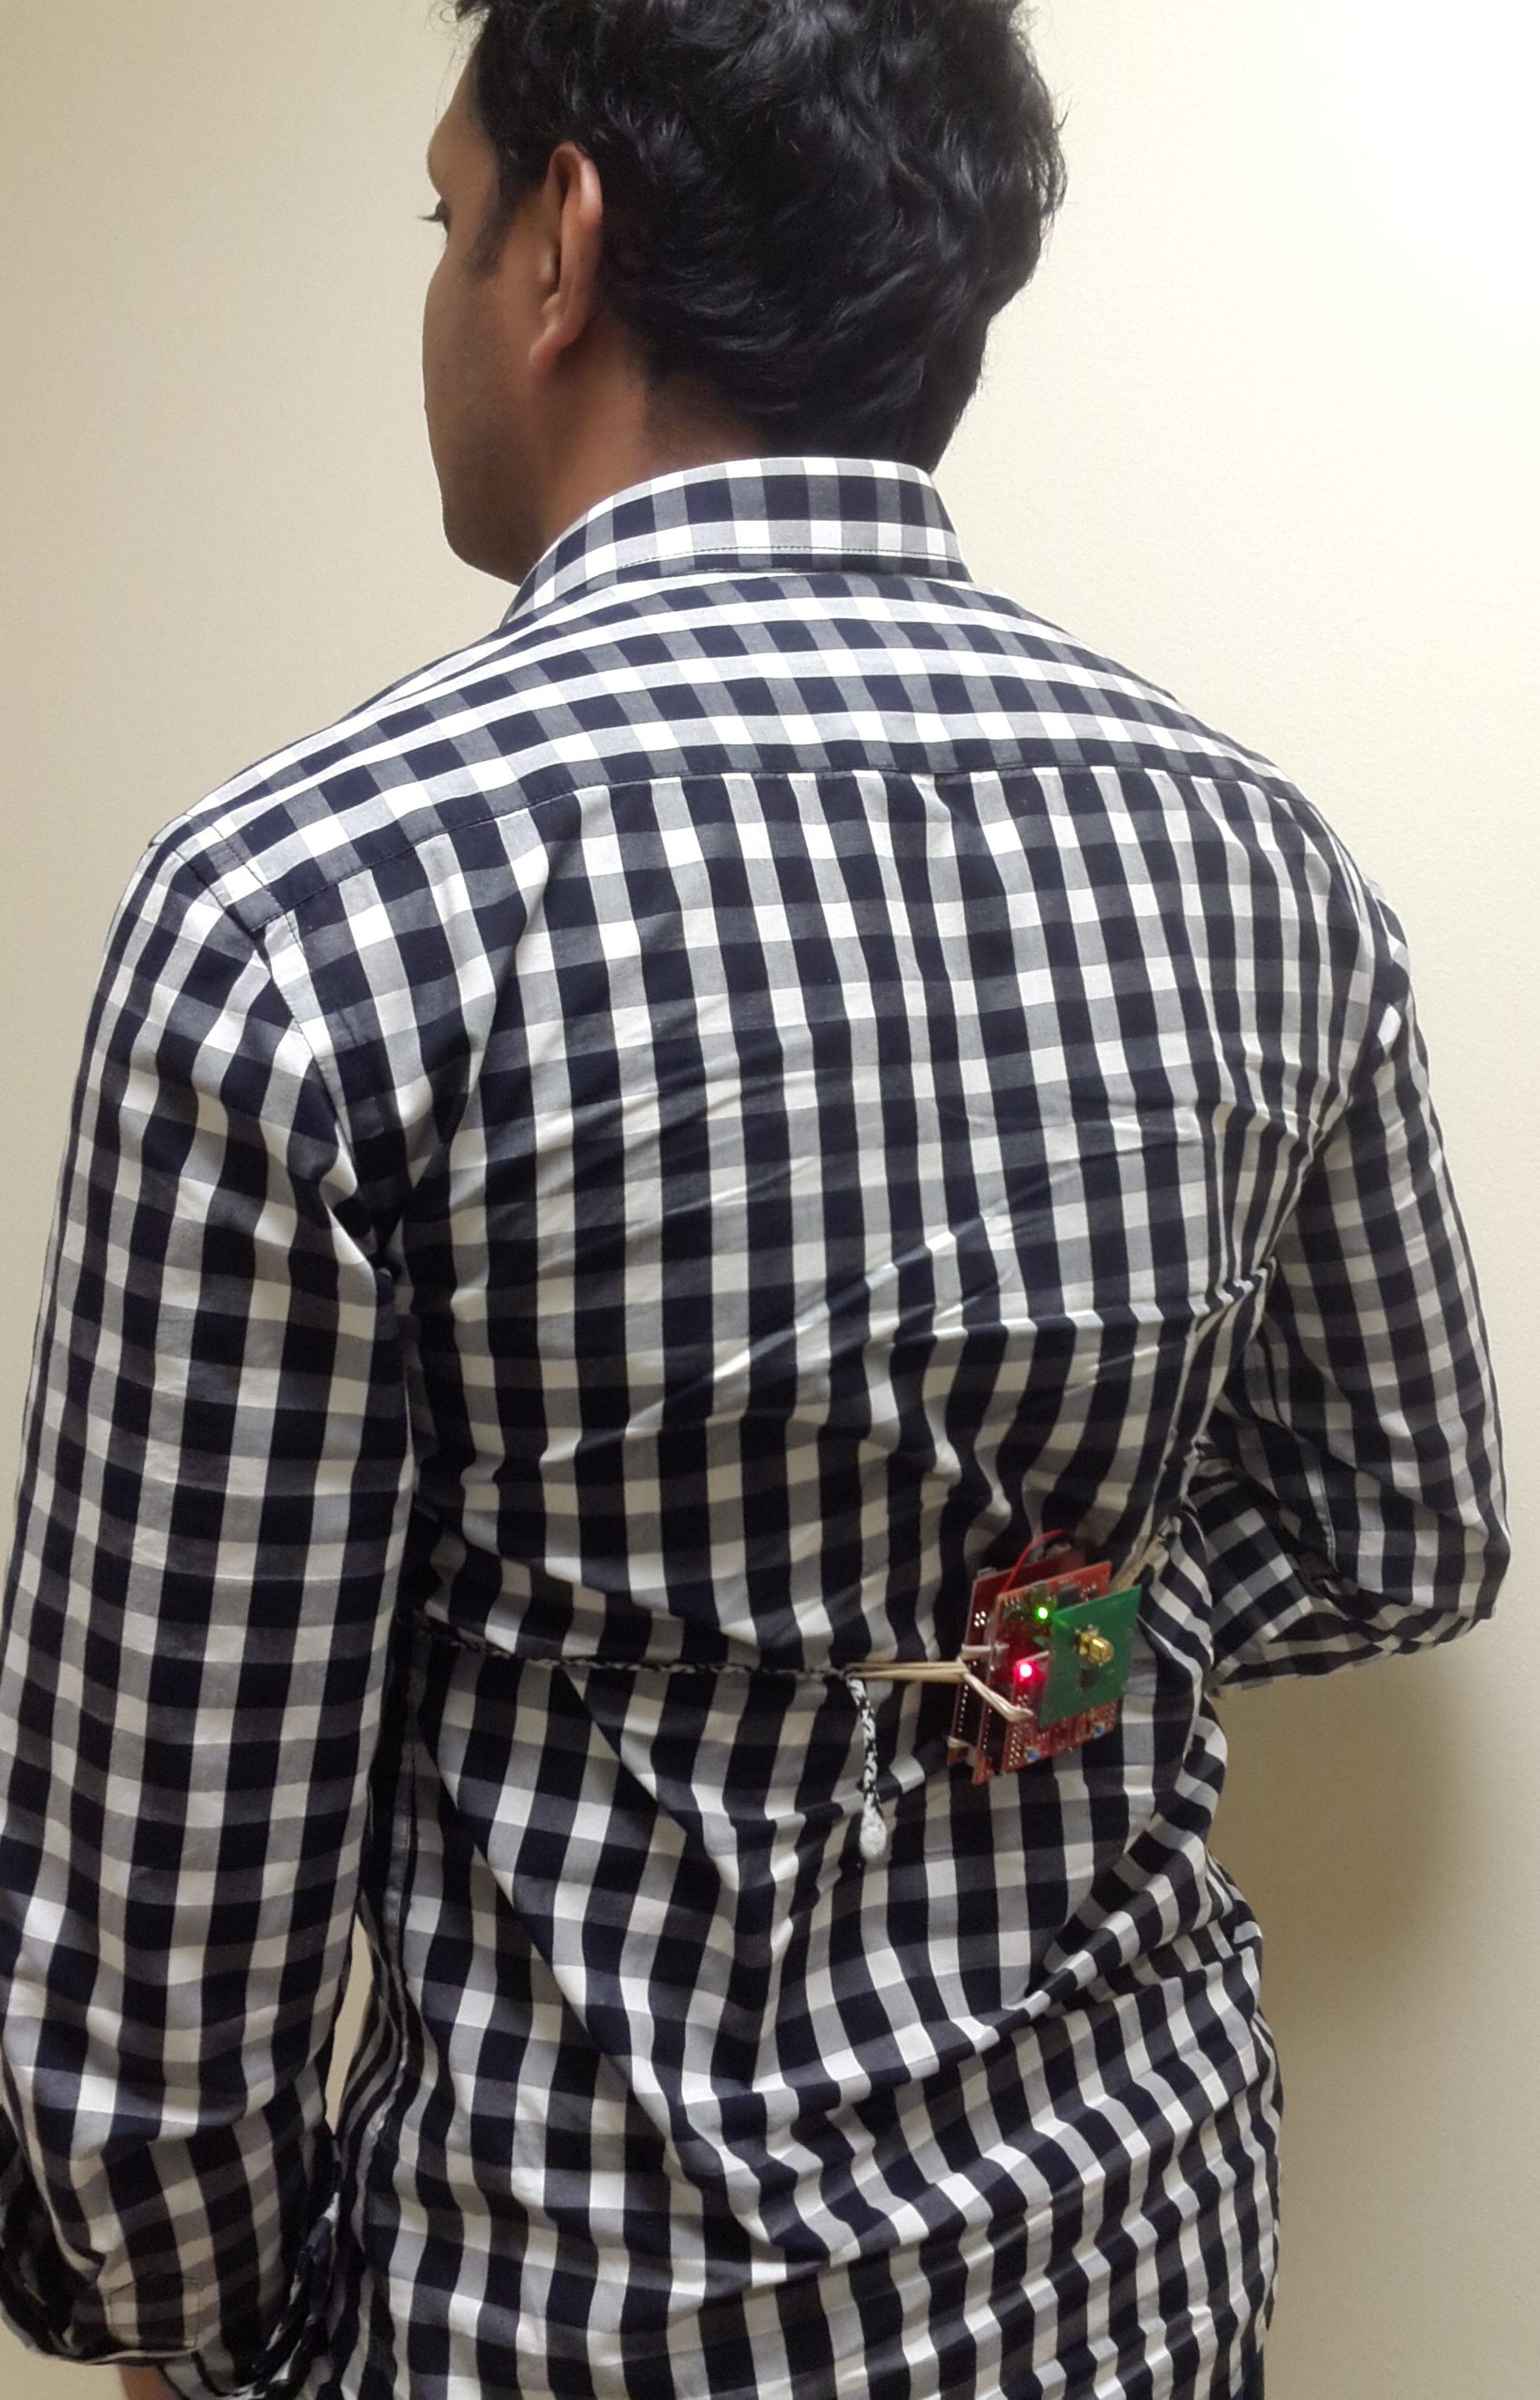
\includegraphics[width=0.21\textwidth]{figures/human_figure}
			\includegraphics[width=0.185\textwidth]{figures/robot_figure}
			\label{fig:framework}
			\caption{(a) Currently available software modules in our framework and a 	directed-graph representation of their functional
				relationship; (b) a wireless sensor device attached to the back of a human subject (c) the same device configuration was used on the back of a NAO
				humanoid robot.}
		\end{figure*}
	\end{block}
}
%%%%%%%%%%%%%%%%%%%%%%%%%%%%%%%%%%%%%%%%%%%%%%%%%%%%%%%%%%%%%



\section{Experimental Setup}
\subsection{Activity Annotation}

\subsubsection*{Activity Annotation}
\frame{
	\frametitle{Experimental Setup}
	\setbeamercovered{transparent} 
	\begin{block}{Activity Annotation}
		\begin{figure*}
			\includegraphics[width=0.25\textwidth]{plots/human_walk2-crop.pdf}
			\includegraphics[width=0.25\textwidth]{plots/robot_fallen_forward2-crop.pdf}
			\caption{Figures (a) shows 3-axis accelerometer and 3-axis gyroscope graph for human motions walking forward Figures (b) shows 3-axis accelerometer and 3-axis gyroscope graph for robot's fallen forward and backward motions.}
			\label{fig:anotation-human-robot} 
		\end{figure*}
		
	\end{block}
}

%%%%%%%%%%%%%%%%%%%%%%%%%%%%%%%%%%%%%%%%%%%%%%%%%%%%%%%%%%%%%



\section{Evaluation Results}
\subsection{Feature Extraction}
\subsection{Experiments with a Human}
\subsection{Experiments with a NAO Robot}

\subsubsection*{Feature Extraction}
\frame{
	\frametitle{Evaluation Results}
	\setbeamercovered{transparent} 
	\begin{block}{Feature Extraction}
		\begin{itemize}
		\item we sampled with 50$Hz$ sampling rate. 
		\item In order to identify activities: 
		\begin{enumerate} \item we have used a window size of $400ms$ (20 
				samples); and \item we have allowed 10 samples ($200ms$) to overlap between windows. 
			\end{enumerate} 
			\item The selection of the window size is based on the observation that transition from routine  activities to a fall event 
			takes between $180-250ms$. 
			\item Thus, a window size of $400ms$ will include both fall event and 
			non-fall event data for classification
		\end{itemize}
		
	\end{block}
}

%%%%%%%%%%%%%%%%%%%%%%%%%%%%%%%%%%%%%%%%%%%%%%%%%%%%%%%%%%%%%
\subsubsection*{Experiments with a Human}
\frame{
	\frametitle{Evaluation Results}
	\setbeamercovered{transparent} 
	\begin{block}{Experiments with a Human}
		We have conducted twelve motions in total on the human subject. 
		
		\begin{table}[!ht]
			
			\label{tab:human-logistic-class}
			\centering
			\scalebox{0.65}{
				\begin{tabular} {| l | c | c | c| c|| c| c| c| c|}
					\hline
					& \multicolumn{4}{c||}{\bf Logistic regression} & \multicolumn{4}{c|}{\bf SVM classification} \\ 
					\hline
					{\bf Activity} & {\bf  TP}  &	{\bf TN}  &	{\bf FP} &	{\bf FN}& {\bf  TP}  &	{\bf TN}  &	{\bf FP} &	{\bf FN} \\ 
					\hline
					Walking forward	& 91\%	& 90\%	& 10\%	& 9\% & 96\%	& 93\%	& 7\%	& 4\% \\ \hline
					Walking backward	& 82\%	& 86\%	& 14\%	& 18\% & 81\%	& 84\%	& 16\%	& 19\% \\ \hline
					Walking left 	& 86\%	& 86\%	& 14\%	& 14\% & 89\%	& 90\%	& 10\%	& 11\% \\ \hline
					Walking right 	& 86\%	& 86\%	& 14\%	& 14\% & 89\%	& 90\%	& 10\%	& 11\% \\ \hline
					Falling forward	& 94\%	& 93\%	& 7\%	& 6\% & 96\%	& 93\%	& 7\%	& 4\%	 \\ \hline
					Falling Backward	& 84\%	& 88\%	& 12\%	& 16\%	& 84\%	& 87\%	& 13\%	& 16\% \\ \hline
					Falling left	& 92\%	& 91\%	& 9\%	& 8\%	& 93\%	& 93\%	& 7\%	& 7\% \\ \hline
					Falling Right	& 92\%	& 91\%	& 9\%	& 8\%	& 92\%	& 93\%	& 7\%	& 8\% \\ \hline
					Marching	& 91\%	& 90\%	& 10\%	& 9\%	& 95\%	& 93\%	& 7\%	& 5\% \\ \hline
					Rotate counter-clockwise	& 91\%	& 89\%	& 11\%	& 9\%	& 93\%	& 91\%	& 9\%	& 7\%	 \\ \hline
					Rotate clockwise	& 92\%	& 89\%	& 11\%	& 8\%	& 94\%	& 91\%	& 9\%	& 6\% \\ \hline
					Stand to seat	& 96\%	& 92\%	& 8\%	& 4\%	& 96\%	& 92\%	& 8\%	& 4\%	 \\ \hline
				\end{tabular}
			}
			\caption{Logistic regression and SVM classification for human activities.}
		\end{table}
		
	\end{block}
}


%%%%%%%%%%%%%%%%%%%%%%%%%%%%%%%%%%%%%%%%%%%%%%%%%%%%%%%%%%%%%
\subsubsection*{Experiments with a NAO Robot}
\frame{
	\frametitle{Evaluation Results}
	\setbeamercovered{transparent} 
	\begin{block}{Kalman Filtering}
		\begin{itemize}
			\item To threshold-based decision making, we have filtered the roll, pitch, and
			yaw values using a Kalman filter.
			
			\item The thresholding method suggests that, if the filtered roll values are within $[90\pm15^{\circ}]$ and the filtered pitch values are within  $[0\pm15]^{\circ}$, then with 100\% 
			accuracy, the NAO  robot will be in a normal state. Otherwise the robot 
			is in a fallen state.
			\item If the filtered roll value is less that $60^{\circ}$ 
			, we can safely assume that the robot is falling forward. If the filtered roll values is 
			more than 100$^{\circ}$ we can assume that the robot is falling backward.
			\item  With these thresholds for a separate test cases, the thresholding method has detected fallen 
			state with 100\% accuracy. 
		\end{itemize}
	\end{block}
}

%%%%%%%%%%%%%%%%%%%%%%%%%%%%%%%%%%%%%%%%%%%%%%%%%%%%%%%%%%%%%
\subsubsection*{Experiments with a NAO Robot}
\frame{
	\frametitle{Evaluation Results}
	\setbeamercovered{transparent} 
	\begin{block}{Kalman Filtering}
		\begin{figure*}
			\includegraphics[width=0.25\textwidth]
				{figures/plot1-crop}
			\includegraphics[width=0.25\textwidth]
				{figures/plot5-crop}
			\includegraphics[width=0.25\textwidth]
				{figures/plot1_fallen-crop}
			\includegraphics[width=0.25\textwidth]
				{figures/plot2_fallen-crop}
			\caption{Figures (a--b) show the roll and pitch angles (raw and filtered) for normal 
				behaviors marching in place and walking backward. Figures (c--d) show the raw and filtered roll 
				and pitch angles for fallen forward and backwards states of NAO humanoid robot.}
			\label{fig:normalFallenBehavior}
		\end{figure*}
	\end{block}
}

%%%%%%%%%%%%%%%%%%%%%%%%%%%%%%%%%%%%%%%%%%%%%%%%%%%%%%%%%%%%%
\subsubsection*{Experiments with a NAO Robot}
\frame{
	\frametitle{Evaluation Results}
	\setbeamercovered{transparent} 
	\begin{block}{Experiments with a NAO Robot}
		We have conducted eleven motions in total on the robot subject. 
		\begin{table}[!ht]
			
			\label{tab:robot-logistic-class}
			\centering
			\scalebox{0.65}{
				\begin{tabular} {| l | c | c | c| c|| c| c| c| c|}
					\hline
					& \multicolumn{4}{c||}{\bf Logistic regression} & \multicolumn{4}{c|}{\bf SVM classification} \\ 
					\hline
					{\bf Activity} & {\bf  TP}  &	{\bf TN}  &	{\bf FP} &	{\bf FN}& {\bf  TP}  &	{\bf TN}  &	{\bf FP} &	{\bf FN} \\ 
					\hline
					Walking forward	& 91\%	& 90\%	& 10\%	& 9\% & 93\%	& 91\%	& 9\%	& 7 \% \\ \hline
					Walking backward	& 90\%	& 90\%	& 10\%	& 10\% & 93\%	& 91\%	& 9\%	& 7\% \\ \hline
					Walking left 	& 92\%	& 90\%	& 10\%	& 8\%  & 94\%	& 90\%	& 10\%	& 6\% \\ \hline
					Walking right 	& 89\%	& 90\%	& 10\%	& 11\% & 90\%	& 91\%	& 9\%	& 10\% \\ \hline
					Falling forward	& 94\%	& 93\%	& 7\%	& 6\%	& 98\%	& 93\%	& 7\%	& 2\% \\ \hline
					Falling Backward	& 94\%	& 93\%	& 7\%	& 6\%	 & 98\%	& 93\%	& 7\%	& 2\% \\ \hline
					Falling left	& 95\%	& 93\%	& 7\%	& 5\%	& 99\%	& 94\%	& 6\%	& 1\% \\ \hline
					Falling Right	& 94\%	& 93\%	& 7\%	& 6\%	& 98\%	& 93\%	& 7\%	& 2\%	 \\ \hline
					Marching	& 91\%	& 89\%	& 11\%	& 9\%	& 90\%	& 91\%	& 11\%	& 10\%	 \\ \hline
					Rotate counter-clockwise	& 97\%	& 92\%	& 8\%	& 3\%	& 97\%	& 93\%	& 7\%	& 3\%	 \\ \hline
					Rotate clockwise	& 98\%	& 92\%	& 8\%	& 2\%	& 96\%	& 93\%	& 7\%	& 4\%	 \\ \hline
				\end{tabular}
			}
			\caption{Logistic regression  and SVM classification for robot activities.}
		\end{table}
		
	\end{block}
}

%%%%%%%%%%%%%%%%%%%%%%%%%%%%%%%%%%%%%%%%%%%%%%%%%%%%%%%%%%%%%

\section{Conclusion \& Future Work}
\subsubsection*{Conclusion \& Future Work}

\frame{
	\frametitle{Conclusion \& Future Work}
	\setbeamercovered{transparent} 
	\begin{block}{Conclusion \& Future Work}
		\begin{itemize}
		 \item	We proposed methods to learn and predict different activities
			for humans and robots;
		\item We also developed a framework software tools to realize these functions on embedded devices.
		\item We were able to detection of falls and other activities for both humans and
			robots within a unified framework with $91\%-100\%$ accuracy;
		\item our future work will be to use multiple sensing devices to create a sensor network to detect complex activities with higher sampling rates.
		\end{itemize}
		
	\end{block}
}


%%%%%%%%%%%%%%%%%%%%%%%%%%%%%%%%%%%%%%%%%%%%%%%%%%%%%%%%%%%%%

\section{*Conclusion \& Future Work}
\subsubsection*{*Conclusion \& Future Work}

\frame{
	\frametitle{}
	\setbeamercovered{transparent} 
	\begin{block}{}
		\centering
			\huge Thanks for listening
	\end{block}
}

%%%%%%%%%%%%%%%%%%%%%%%%%%%%%%%%%%%%%%%%%%%%%%%%%%%%%%%%%%%%%

\section{*Conclusion \& Future Work}
\subsubsection*{*Conclusion \& Future Work}

\frame{
	\frametitle{}
	\setbeamercovered{transparent} 
	\begin{block}{}
		\centering
		\huge Questions ?
	\end{block}
}

\end{document}